\documentclass[aspectratio=169]{beamer}
\usepackage{standalone}

\usepackage{stmaryrd}
\usepackage{listings}
\usepackage{bussproofs}

\usepackage[hyperref=auto,style=alphabetic,backend=bibtex]{biblatex}
\addbibresource{kwarcpubs.bib}
\addbibresource{extpubs.bib}
\addbibresource{extcrossrefs.bib}
\usepackage{appendixnumberbeamer}
\usepackage{tikz}
\usepackage{tikz-qtree}
\usepackage{mdframed}
\usetikzlibrary{arrows.meta}
\usetikzlibrary{mmt}
\usetikzlibrary{docicon}

\usetheme{Pittsburgh}
\setbeamertemplate{footline}[frame number]
\setbeamertemplate{navigation symbols}{}
\usecolortheme{beaver}
\setbeamertemplate{frametitle}[default][left]
% \setbeamersize{text margin left=3em}

% \usepackage{courier}
\usepackage{fontspec}
\setmonofont[Scale=MatchLowercase]{Consolas}

\usepackage{utils/colors}
\usepackage{utils/basic}
\usepackage{utils/operators}
\usepackage{utils/mylstmisc}
\usepackage{utils/lstmmt}

\lstset{basicstyle=\ttfamily}
\lstset{commentstyle=\itshape\color{commentfont}}

\title{Prototyping Natural Language Understanding with GF \\ \large  Adding Semantics and Inference}

\author{Jan Frederik Schaefer}
\institute{FAU Erlangen-N\"urnberg}
\date{\textbf{GF Summer School 2021} \\ \textit{Singapore/online} \\ August 2, 2021 }

\begin{document}
\frame\titlepage

\begin{frame}
    \frametitle{\itshape whoami}
    \begin{itemize}
        \item Just started my PhD (\textit{Semantics Extraction in STEM})
        \item FAU ({\bf F}riedrich-{\bf A}lexander-{\bf U}niversit\"at Erlangen-N\"urnberg) in Germany
        \item KWARC research group:
            \begin{itemize}
                \item Led by Michael Kohlhase
                \item Knowledge representation and reasoning techniques
                \item Focus on mathematical content
            \end{itemize}
    \end{itemize}
    
    \vspace{1.5em}
    \begin{columns}[T]
        \begin{column}{0.45\textwidth}
            \textbf{Talk in Stellenbosch:}\\
            \begin{itemize}
                \item GF + MMT for semantics
                \item Mathematical language
            \end{itemize}
        \end{column}
        \begin{column}{0.45\textwidth}
            \textbf{Today:}\\
            \begin{itemize}
                \item Extended and more mature system
                \item Less mathematical language
            \end{itemize}
        \end{column}
    \end{columns}

\end{frame}

\begin{frame}
    \frametitle{Method of Fragments}
    \only<1-2>{
        \centering
        \only<1>{\def\fraglevel{0}}
        \only<2>{\def\fraglevel{1}}
        \includestandalone{fig/montague-fragments}

        \begin{minipage}[t][2cm]{\textwidth}\vspace{1em}
            How do we get from messy language to formal logic?\\[0.5em]
            \emph{Montague}~\cite{Montague:efl70}: Look at a ``nice'' subset
            and map into logic.
        \end{minipage}
    }

    \only<3>{
        \centering
        \def\fraglevel{1}
        \includestandalone{fig/montague-fragments}
        
        \begin{minipage}[t][2cm]{0.6\textwidth}\vspace{1em}
            \str{Ahmed paints and Berta is quiet.}\\[0.5em]
            \str{Ahmed doesn't paint.}
        \end{minipage}\hfill
        \begin{minipage}[t][2cm]{0.39\textwidth}\vspace{1em}
            $p(a) \wedge q(b)$\\[0.5em]
            $\neg p(a)$
        \end{minipage}
    }

    \only<4>{
        \centering
        \def\fraglevel{2}
        \includestandalone{fig/montague-fragments}
        
        \begin{minipage}[t][2cm]{0.6\textwidth}\vspace{1em}
            \str{Every student paints and is quiet.}\\[0.5em]
            \str{Nobody paints.}
        \end{minipage}\hfill
        \begin{minipage}[t][2cm]{0.39\textwidth}\vspace{1em}
            $\forall x.s(x) \Rightarrow (p(x) \wedge q(x))$\\[0.5em]
            $\neg \exists x.p(x)$
        \end{minipage}
    }

    \only<5>{
        \centering
        \def\fraglevel{3}
        \includestandalone{fig/montague-fragments}

        \begin{minipage}[t][2cm]{0.6\textwidth}\vspace{1em}
            \str{Ahmed isn't allowed to paint.}\\[0.5em]
            \str{Ahmed and Berta must paint.}
        \end{minipage}\hfill
        \begin{minipage}[t][2cm]{0.39\textwidth}\vspace{1em}
            $\neg\lozenge p(a)$\\[0.5em]
            $(\square p(a)) \wedge \square p(b)$
        \end{minipage}
    }
\end{frame}


\begin{frame}
    \frametitle{Method of Fragments}
    {\color{hlfont}Hand-waving} is problematic:

    \hspace{2em}\str{Ahmed paints. He is quiet.}
    {$\quad\stackrel{?}{\leadsto}\quad$ \color{logicfont} $p(a)\wedge q(a)$}

    \vspace{1.2em}
    {\color{hlfont}Montague}: Specify
    \begin{itemize}
        \item grammar,\com{fixes NL subset}
        \item target logic,
        \item semantics construction.\com{maps parse trees to logic}
    \end{itemize}

    {
        \centering
        \vspace{0.3em}
        {\itshape\footnotesize Example from~\cite{Montague:tptoqi73}}

        \vspace{0.2em}\fbox{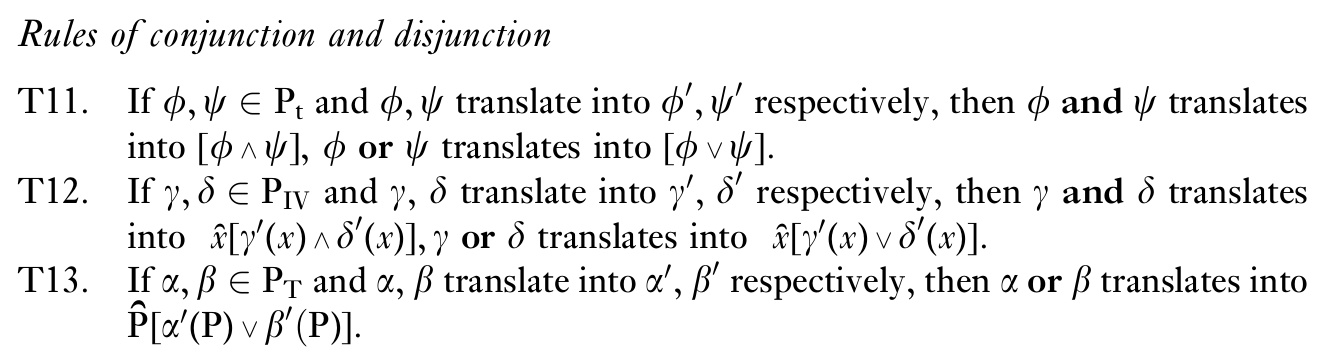
\includegraphics[trim=0 0 0 80,clip,width=0.7\textwidth]{fig/montague-tptoqioe.png}}

        \vspace{1.2em}
        Claim: That doesn't scale well $\leadsto$ \textbf{We need {\color{hlfont}prototyping}!}
    }

    % \newcommand\VP{\text{\upshape\tiny VP}}
    % \hspace{2em}$\llbracket\text{\strplain{$P_{\VP}$ and $Q_{\VP}$}}\rrbracket_{\VP} = \lambda x. \llbracket\text{\strplain{$P_{\VP}$}}\rrbracket(x) \wedge \llbracket\text{\strplain{$Q_{\VP}$}}\rrbracket(x)$
\end{frame}


\def\gfsemconstrpicAST{$\text{AST}$}
\def\gfsemconstrpicLOG{$\text{String}_\text{Logic}$}
\def\gfsemconstrpicArrow{\ttfamily linearize}
\def\gfsemconstrpic{
    {\centering
        \begin{tikzpicture}[xscale=1.2]
            \tikzset{ll/.style={line width=0.7pt}}
            \draw[ll,fill=nlbg] (-5.0,-0.5) rectangle (-3.0,0.5);
            \draw[ll,fill=nlbg!50!logicbg] (-1.0,-0.5) rectangle (1.0,0.5);
            \draw[ll,fill=logicbg] (3.0,-0.5) rectangle (5.0,0.5);
            \node[] at (-4.0, 0.0) {$\text{String}_\text{Eng}$};
            \node[] at (0.0, 0.0) {\gfsemconstrpicAST};
            \node[] at (4.0, 0.0) {\gfsemconstrpicLOG};
            \draw[ll, ->] (-3,0) to node[above]{\footnotesize \ttfamily parse} (-1,0);
            \draw[ll, ->] (1,0) to node[above]{\footnotesize \gfsemconstrpicArrow} (3,0);
        \end{tikzpicture}\par}
}

\begin{frame}
    \frametitle{Method of Fragments}
    \textbf{How can we implement such fragments (with the help of GF)?}

    \vspace{0.5em}
    \begin{itemize}
        \item Use GF for parsing
        \item 4 ideas how to continue
    \end{itemize}

    \vspace{1.5em}

    \def\gfsemconstrpicAST{$\text{AST}$}
    \def\gfsemconstrpicArrow{???}
    \def\gfsemconstrpicLOG{???}
    \gfsemconstrpic{}
\end{frame}


\begin{frame}[fragile]
    \frametitle{Idea 1: Concrete Syntax for Logic}
    \gfsemconstrpic{}

    \vspace{0.5em}
    \only<1-2>{
        \lstinline[language=GLIFcmd,stringstyle=\color{nlfg},keepspaces=true]!parse -lang=Eng "Ahmed paints and Berta is quiet" | linearize -lang=Logic!\\
        {\color{logicfg}\ttfamily p ( a ) \lstmmtboldmath$\wedge$ q ( b )}
    }
    \only<3-4>{
        \lstinline[language=GLIFcmd,stringstyle=\color{nlfg},keepspaces=true]!parse -lang=Eng "Ahmed is quiet and paints" | linearize -lang=Logic!\\
        \only<3>{\color{hlfg}\ttfamily q ( a ) \lstmmtboldmath$\wedge$ p ( a ) ???}
        \only<4>{\color{logicfg}\ttfamily (λx. q (x) \lstmmtboldmath$\wedge$ p (x)) ( a )\com{$\leadsto_\beta q(a)\wedge p(a)$}}
    }

    \onslide<2-4>{
    \begin{columns}[t]
        \begin{column}{0.38\textwidth}
            \begin{mdframed}[backgroundcolor=logicbg!50!nlbg, innerleftmargin=2.5, innerrightmargin=0.2, innertopmargin=0.2,innerbottommargin=0.2, outerlinewidth=0.7]
                \only<1-3>{\onslide<2-3>{
                    \footnotesize\lstinputlisting[linewidth=6.0cm,language=GF]{slides/misc/snippets/s006.txt}
                }}
                \only<4>{
                    \footnotesize\lstinputlisting[linewidth=6.0cm,language=GF]{slides/misc/snippets/s008.txt}
                }
            \end{mdframed}
        \end{column}
        \begin{column}{0.54\textwidth}
            \begin{mdframed}[backgroundcolor=logicbg, innerleftmargin=2.5, innerrightmargin=0.2, innertopmargin=0.2,innerbottommargin=0.2, outerlinewidth=0.7]
                \only<1-3>{\onslide<2-3>{
                    \footnotesize\lstinputlisting[linewidth=6.0cm,language=GF,alsoletter={\\},literate={\\wedge}{\lstmmtboldmath$\wedge$}1,stringstyle=\color{logicfg}]{slides/misc/snippets/s007.txt}
                }}
                \only<4>{
                    \footnotesize\lstinputlisting[linewidth=6.0cm,language=GF,alsoletter={\\},literate={\\wedge}{\lstmmtboldmath$\wedge$}1{\\lambda}{$\uplambda$}1,stringstyle=\color{logicfg}]{slides/misc/snippets/s009.txt}
                }
            \end{mdframed}
        \end{column}
    \end{columns}
    }
\end{frame}

\begin{frame}[fragile]
    \frametitle{Idea 2: Abstract Syntax for Logic}
    \def\gfsemconstrpicAST{$\text{AST}_\text{NL}$}
    \def\gfsemconstrpicArrow{\ttfamily pt -compute}
    \def\gfsemconstrpicLOG{$\text{AST}_\text{Logic}$}
    \gfsemconstrpic{}

    \begin{columns}[t]
        \begin{column}{0.42\textwidth}
            \begin{mdframed}[backgroundcolor=logicbg, innerleftmargin=2.5, innerrightmargin=0.2, innertopmargin=0.2,innerbottommargin=0.2, outerlinewidth=0.7]
                \footnotesize\lstinputlisting[linewidth=3.5cm,language=GF]{slides/misc/snippets/s010.txt}
            \end{mdframed}
        \end{column}
        \begin{column}{0.58\textwidth}
            \onslide<2-3>{
                \begin{mdframed}[backgroundcolor=white, innerleftmargin=2.5, innerrightmargin=0.2, innertopmargin=0.2,innerbottommargin=0.2, outerlinewidth=0.7]
                    \footnotesize\lstinputlisting[linewidth=6.0cm,language=GF]{slides/misc/snippets/s011.txt}
                \end{mdframed}
            }
        \end{column}
    \end{columns}

    \vspace{1.0em}
    \onslide<3>{
        \lstinline[language=GLIFcmd,stringstyle=\color{nlfg},keepspaces=true]!parse -lang=Eng -cat=Prop "Ahmed is quiet and paints" | put_tree -compute!\\
        {\color{logicfg}\ttfamily and (q a) (p a)}
    }
\end{frame}

\begin{frame}
    \frametitle{All 4 Ideas}
    \begin{enumerate}
        \item \textbf{Use another concrete syntax:}\par
            \gfsemconstrpic{}
        \item \textbf{Use another abstract syntax:}\par
            \def\gfsemconstrpicAST{$\text{AST}_\text{NL}$}
            \def\gfsemconstrpicArrow{\ttfamily pt -compute}
            \def\gfsemconstrpicLOG{$\text{AST}_\text{Logic}$}
            \gfsemconstrpic{}
        \pause
        \item \textbf{Use a general-purpose programming language:}\par
            \def\gfsemconstrpicAST{$\text{AST}$}
            \def\gfsemconstrpicArrow{process with}
            \def\gfsemconstrpicLOG{Haskell}
            \gfsemconstrpic{}
        \pause
        \item \textbf{Use a logic development framework:}\par
            \def\gfsemconstrpicAST{$\text{AST}$}
            \def\gfsemconstrpicArrow{process with}
            \def\gfsemconstrpicLOG{MMT}
            \gfsemconstrpic{}
    \end{enumerate}
\end{frame}


\begin{frame}
    \frametitle{MMT}
    \begin{itemize}
        \item Tool for logic development and knowledge representation
        \item ``Bring your own logic''
        \item Implement syntax, semantics, calculi
        \item Lots of logics already implemented\com{LATIN2 project}
        \item Supports type theory underlying GF
        \item Developed by KWARC group\com{we are biased towards MMT}
        \item Three steps:
            \begin{enumerate}
                \item Represent abstract syntax in MMT\com{is automated}
                \item Declare target logic
                \item Declare mapping from 1.\ to 2.
            \end{enumerate}
    \end{itemize}
\end{frame}

\begin{frame}
    \frametitle{MMT}
    \begin{enumerate}
        \item {\only<1>{\color{hlfg}\bfseries} Represent abstract syntax in MMT}\com{is automated}
        \item {\only<2-3>{\color{hlfg}\bfseries} Declare target logic}
        \item {\only<4>{\color{hlfg}\bfseries} Declare mapping from 1.\ to 2.}
    \end{enumerate}

    \begin{columns}[t]
        \only<1>{
            \begin{column}{0.48\textwidth}
                \footnotesize\lstinputlisting[linewidth=6.0cm,language=GF]{slides/misc/snippets/s012.txt}
            \end{column}
            \begin{column}{0.48\textwidth}
                \footnotesize\lstinputlisting[linewidth=6.0cm,language=MMT]{slides/misc/snippets/s013.txt}
            \end{column}
        }
        \only<2-3>{
            \begin{column}{0.43\textwidth}
                \footnotesize\lstinputlisting[linewidth=6.0cm,language=MMT]{slides/misc/snippets/s014.txt}
            \end{column}
            \begin{column}{0.53\textwidth}
                \only<3>{
                    \footnotesize\lstinputlisting[linewidth=6.0cm,language=MMT]{slides/misc/snippets/s015.txt}
                }
            \end{column}
        }
        \only<4>{
            \begin{column}{0.5\textwidth}
                \footnotesize\lstinputlisting[linewidth=6.0cm,language=MMT]{slides/misc/snippets/s016.txt}
            \end{column}
        }
    \end{columns}
    \vspace{10cm}\par
\end{frame}



\begin{frame}
    \frametitle{GLIF: The Grammatical Logical Inference Framework}
    \centering
    \only<1-3>{
        \disablepart{elpibox}
        \disablepart{sempragarrow}
    }
    \includestandalone[width=0.9\textwidth]{fig/glif-architecture}

    \only<2>{
        \begin{tikzpicture}[overlay,remember picture]
            \fill[gray!80,opacity=0.8] (current page.north west) rectangle (current page.south east);
            \node at (current page.center) { 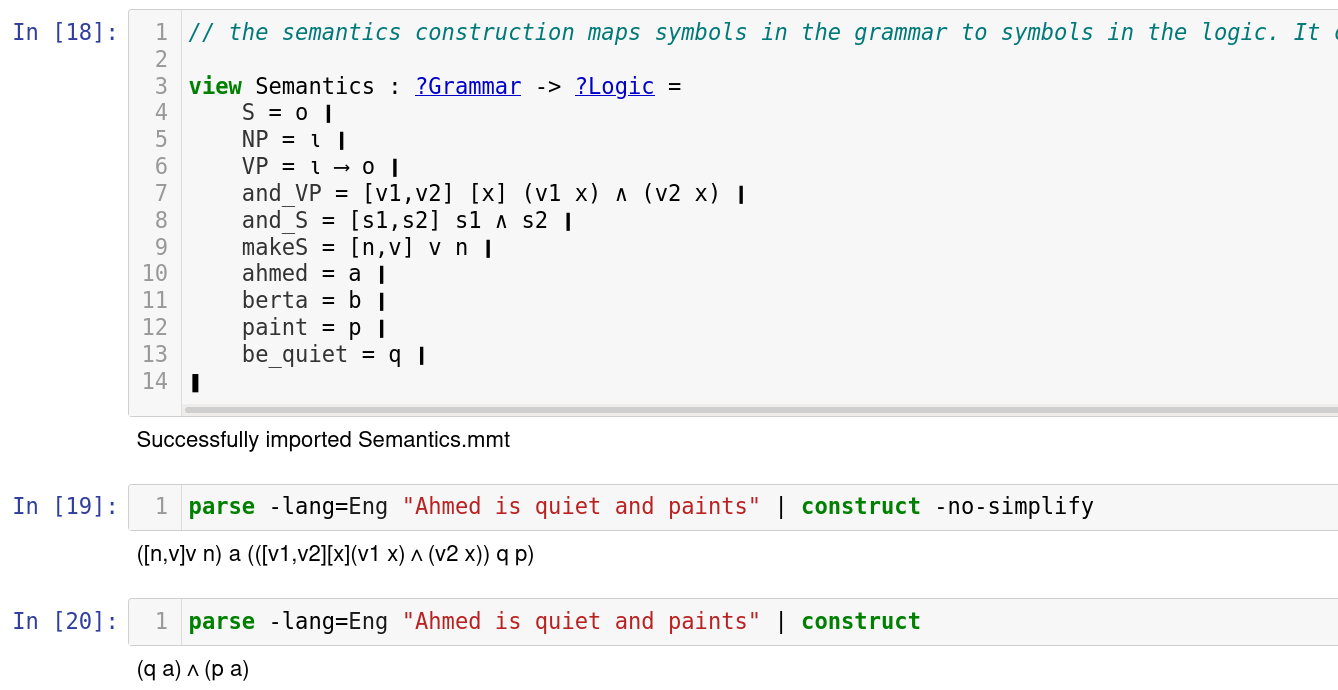
\includegraphics[width=0.85\textwidth]{img/screenshot-glif-2.png} };
        \end{tikzpicture}
    }

    \vspace{1.5em}
    \onslide<4>{
        \setlength{\arrayrulewidth}{1.0pt}
        \begin{tabular}{r@{\hskip3pt} l l}
            \vspace{0.1em} &\textbf{GF}   &{(= \textbf{grammar} framework)}\\
            \vspace{0.1em}+&\textbf{MMT}  &{(= \textbf{logic} framework)}\\
            \vspace{0.1em}+&\textbf{ELPI} &{(= \textbf{inference} framework)}\\
            \hline
            \\[-1em]
            =&\textbf{GLIF} &{(= \textbf{natural language understanding} framework)}\\
        \end{tabular}
    }
\end{frame}

% \begin{frame}
    \frametitle{Example: Controlled Natural Languages}
    \begin{itemize}
        \item Formal languages
        \item that are a subset of natural language
        \item and have fixed semantics\com{formal verification, \dots}
    \end{itemize}

    \vspace{1em}
    \str{$S$ is a subset of every set iff $S$ is empty}

    $\leadsto$ {\color{logicfont}$(\forall V_{new}. set(V_{new}) \Rightarrow subset(V_S, V_{new})) \Leftrightarrow empty(V_S)$}

    \pause
    \vspace{1.5em}
    Use inference for disambiguation:

    \vspace{1em}
    \only<2>{\disablepart{crossout}}
    \only<3>{\enablepart{crossout}}
    \includestandalone[width=\textwidth]{fig/cnl-simple-discard} 
\end{frame}

\provideenablepart{aselpientro}
\def\ifelpi#1#2{\ifpart{aselpientro}{#1}{#2}}

\begin{frame}
    \ifpart{aselpientro}{
        \frametitle{ELPI}
        \begin{itemize}
            \item Extension of $\lambda$Prolog\com{supports higher-order abstract syntax}
            \item Generic inference/reasoning step after semantics construction
            \item Goal: Use it for semantic/pragmatic analysis
        \end{itemize}
    }{\frametitle{Example: Discard wrong readings in controlled natural language}}

    \begin{minipage}[t][4cm][t]{\textwidth}
        \ifpart{aselpientro}{
            \pause
            \vspace{2em}
            Example: Discard wrong readings in controlled natural language

            \vspace{1em}
        }{}
        \only<\ifelpi2{1-4}>{
            \tikzset{every picture/.style={line width=0.7pt}}
            \begin{tikzpicture}[yscale=0.5]
                \node(str0) at (-4,0) {\str{the ball has a mass of 5kg}};
                \node(ast0) at (-0.5,0) {AST};
                \node(log0) at (4,0) {\ifcolorful\color{logicfont}\fi$\text{mass}(\text{theball}, \text{quant}(5, \text{kilo gram}))$};
                \draw[-{Straight Barb[length=6.3,width=5.0]},gray] (str0) -- (ast0);
                \draw[-{Straight Barb[length=6.3,width=5.0]},gray] (ast0) -- (log0);
            \end{tikzpicture}
            \vspace{3em}
        }
        \only<\ifelpi32>{\disablepart{crossout}}
        \only<\ifelpi4{3-4}>{\enablepart{crossout}}
        \enablepart{switchtonmexample}
        \onslide<\ifelpi{3-4}{2-4}>{
            \includestandalone[width=\textwidth]{fig/cnl-simple-discard} 
        }
    \end{minipage}

    \only<\ifelpi54>{
        \begin{tikzpicture}[overlay,remember picture]
            \fill[gray!80,opacity=0.8] (current page.north west) rectangle (current page.south east);
            \node at (current page.center) { 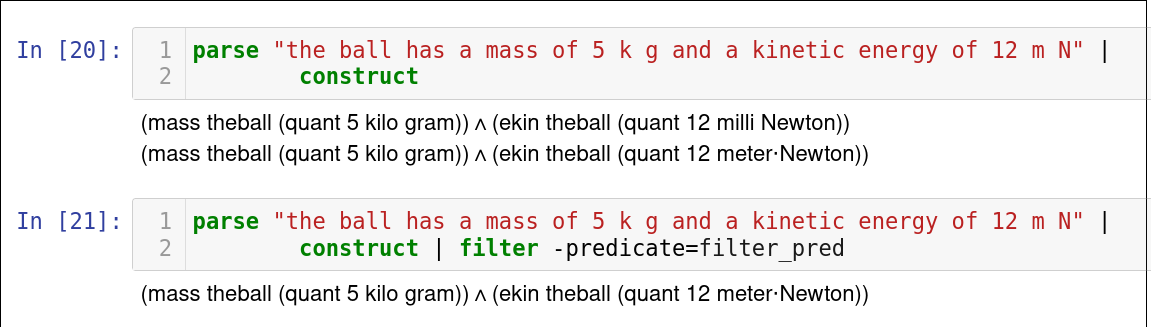
\includegraphics[width=0.95\textwidth]{img/screenshot-glif-3.png} };
        \end{tikzpicture}
    }
\end{frame}


\begin{frame}
    \frametitle{Example: ``pairwise disjoint''}
    \newcommand\ds{\text{disjoint}}
    \str{$A$, $B$ and $C$ are pairwise disjoint}\\
    {\color{logicfont} $\ds(A,B) \wedge \ds(A,C) \wedge \ds(B,C)$}
    \vspace{1em}

    \begin{itemize}
        \item \textbf{Approach 1}\\Semantics construction with lots of $\lambda$s:\com{difficult!}
            {\hspace{2em}\color{logicfont} $\ds(A,B) \wedge \ds(A,C) \wedge \top \wedge \ds(B,C) \wedge \top \wedge \top\wedge\top$}\\
                Simplify with ELPI:\\
            {\hspace{2em}\color{logicfont} $\ds(A,B) \wedge \ds(A,C) \wedge \ds(B,C)$}
        \pause
        \item \textbf{Approach 2}\\Semantics construction creates preliminary expression:\\
            {\hspace{2em}\color{logicfont}\ttfamily relNT disjoint (cons A (cons B (cons C nil))) }\\
                Convert with ELPI:\com{easier}
            {\hspace{2em}\color{logicfont} $\ds(A,B) \wedge \ds(A,C) \wedge \ds(B,C)$}
    \end{itemize}
\end{frame}

\begin{frame}
    \frametitle{The ``Normal'' GLIF Pipeline}
    \includestandalone[width=\textwidth]{fig/glif-architecture}
\end{frame}

\enablepart{showscreenshot}
\begin{frame}[fragile]
    \def\mybox#1{\square_{#1}}
    \def\mydia#1{\lozenge_{#1}}
    \def\sfiven{{S5_n}}
    \frametitle{Example: Epistemic Q\&A}
    \centering
    \strplain{\makebox[9.5cm][l]{John knows that Mary or Eve knows that Ping has a dog.}\makebox[1.5em]{\upshape($S_1$)}\\
              \makebox[9.5cm][l]{Mary doesn't know if Ping has a dog.}\makebox[1.5em]{\upshape($S_2$)}\\
              \makebox[9.5cm][l]{Does Eve know if Ping has a dog?}\makebox[1.5em]{\upshape($Q$)}}

    {\color{logicfont}
        \begin{align*}
            S_1 &= \mybox{john}(\mybox{mary} hd(ping)\vee \mybox{eve}hd(ping))\\
            S_2 &= \neg(\mybox{mary}hd(ping) \vee \mybox{mary}\neg hd(ping))\\
            Q &= \mybox{eve}hd(ping) \vee \mybox{eve}\neg hd(ping)
        \end{align*}
    }

    \begin{table}
        \begin{tabular}{l l}
            $S_1, S_2 \vdash_\sfiven Q$\quad      &$\leadsto$\quad yes\\
            $S_1, S_2 \vdash_\sfiven \neg Q$\quad &$\leadsto$\quad no\\
            else &$\leadsto$\quad maybe
        \end{tabular}
    \end{table}
\end{frame}


\providedisablepart{showscreenshot}
\begin{frame}[fragile]
    \frametitle{Example: Translation}
    \begin{itemize}
        \item Two German words for \str{cousin}, depending on the gender
        \item Two entries in abstract syntax: \verb|cousin_female| and \verb|cousin_male|
        \item Use inference to discard ASTs
    \end{itemize}
    
    \vspace{2em}
    \small
    \begin{minipage}[t][5cm]{\textwidth}
        \begin{tikzpicture}
            \node(eng) at (-4,1) {\parbox{4.2cm}{\str{Kim is Ahmed's cousin and the father of Grace}}};
                \node(ger1) at (-4,-0.5) {\parbox{4.2cm}{\str{Kim ist Ahmeds {\upshape\bf Cousine} und Graces Vater}}};
                \node(ger2) at (-4,-2.0) {\parbox{4.2cm}{\str{Kim ist Ahmeds {\upshape\bf Cousin} und Graces Vater}}};
            \node(ast1) at (0,1) {AST$_1$};
            \node(ast2) at (0,-1) {AST$_2$};
            \only<2->{
                \node(log1) at (3,1) {\color{logicfont} \parbox{2.2cm}{$female(kim) \wedge$ $male(kim)$}};
                \node(log2) at (3,-1) {\color{logicfont} \parbox{2.2cm}{$male(kim) \wedge$ $male(kim)$}};
            }
            \draw[->,thick] (eng) -- (ast1);
            \draw[->,thick] (eng) -- (ast2);
                \draw[->,thick] (ast1) -- (ger1);
                \draw[->,thick] (ast2) -- (ger2);
            \only<2->{
                \draw[->,thick] (ast1) -- (log1);
                \draw[->,thick] (ast2) -- (log2);
            }
            \only<3>{
                \draw[ultra thick,red] (2,1.5) -- (4,0.5);
                \draw[ultra thick,red] (2,0.5) -- (4,1.5);
                
                \draw[ultra thick,red] (-0.5,1.5) -- (0.5,0.5);
                \draw[ultra thick,red] (-0.5,0.5) -- (0.5,1.5);

                \draw[ultra thick,red] (-6,0.0) -- (-2,-1.0);
                \draw[ultra thick,red] (-6,-1.0) -- (-2,0.0);
            }
        \end{tikzpicture}
    \end{minipage}
    \ifpart{showscreenshot}{\only<4>{
        \begin{tikzpicture}[overlay,remember picture]
            \fill[gray!80,opacity=0.8] (current page.north west) rectangle (current page.south east);
            \node at (current page.center) { 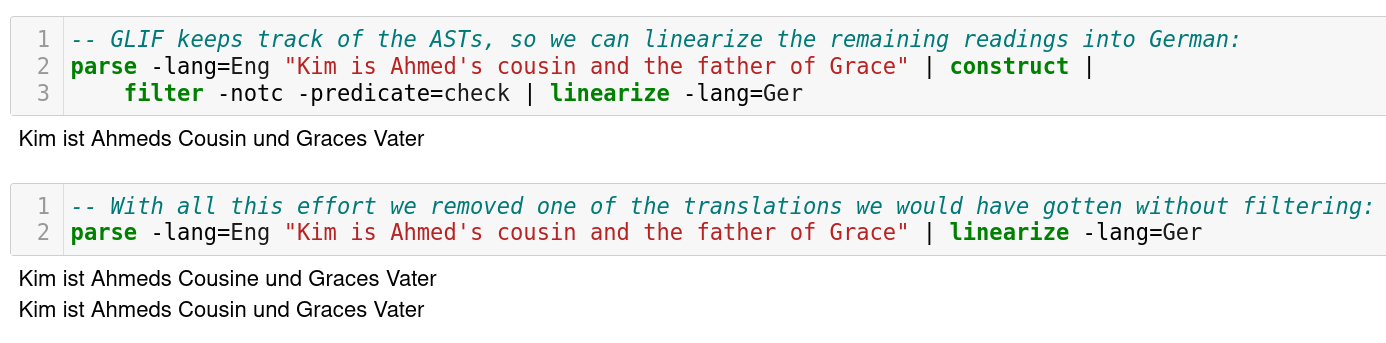
\includegraphics[width=\textwidth]{img/screenshot-glif-5.png} };
        \end{tikzpicture}
    }}{}
\end{frame}


\begin{frame}
    \frametitle{Prover Generation}
    \begin{itemize}
        \item Can describe inference rules in MMT
        \item {\tt $\vdash$X} is the type of proofs of {\tt X}\com{``Judgments as types''}
        \item Example rules:\\
            {\boldmath\tt andEl \ : {\color{black!50}\{A,B\}} $\vdash\,$A$\wedge$B $\rightarrow$ $\vdash\,$A}\\
            {\boldmath\tt andEr \ : {\color{black!50}\{A,B\}} $\vdash\,$A$\wedge$B $\rightarrow$ $\vdash\,$B}\\
            {\boldmath\tt contra : {\color{black!50}\{X\}} $\vdash\,$male(X) $\rightarrow$ $\vdash\,$fem(X) $\rightarrow$ $\lightning$}
        \pause
        \item Generate Prolog/ELPI rules:\\
        {\boldmath\tt
provable(A) \ \ \ \ :- provable(A$\wedge$B).\\
provable(B) \ \ \ \ :- provable(A$\wedge$B).\\
contradiction() :- provable(male(X)), provable(fem(X)).\\
        }
        \item Extra predicates to guide proof search\com{iterative deepening, ...}
    \end{itemize}
\end{frame}


\begin{frame}[fragile]
    \frametitle{Example: Input Language for SageMath}
    \begin{itemize}
        \item Can we make a natural input language for SageMath?\com{WolframAlpha-like}
        % \item Idea: Semantics construction translates to SageMath (not logic)
    \end{itemize}

    \vspace{2.0em}
    {\centering\begin{adjustbox}{}
    \begin{lstlisting}
sage: g = AlternatingGroup(5)
sage: g.cardinality()
60
    \end{lstlisting}
    \end{adjustbox}\par
    \vspace{1.5em}
    \str{Let G be the alternating group on 5 symbols. What is the cardinality of G?}\par
    }
\end{frame}

\begin{frame}
    \frametitle{Example: Input Language for SageMath}
    \centering
    \begin{tikzpicture}[xscale=1.05,yscale=0.9]
        \tikzset{ll/.style={line width=0.7pt}}
            \draw[ll,rounded corners=.2cm,fill=black!20] (-3.4,3.2) rectangle (-0.1,0.0);
            \node at (-1.75,0.5) {\bfseries GF};
            \draw[ll,rounded corners=.2cm,fill=black!20] (0.1,3.2) rectangle (3.4,0.0);
            \node at (1.75,0.5) {\bfseries MMT};
            \draw[ll,rounded corners=.2cm,fill=black!20] (3.6,3.2) rectangle (6.9,0.0);
            \node at (5.25,0.5) {\bfseries GF};
        % rectangle and triangles have same area
        \node[ll,fill=\ifcolorful nlbg\else white\fi,draw=\ifcolorful nlfg\else black\fi,minimum width=1.8cm,minimum height=1cm] (utt) at (-3.5,1.8) {$\text{String}_{NL}$};
        \draw[ll,fill=\ifcolorful nlbg!50!logicbg\else white\fi,draw=\ifcolorful nlfg!50!logicfg\else black\fi] (-1,1) -- (0,3) -- (1,1) -- cycle;
        \node[] (st) at (0,1.5) {$\text{AST}_{NL}$};
        % \usetikzlibrary{arrows.meta}
        \draw[ll,-{Straight Barb[length=6.3,width=5.0]}] (-2.5, 1.8) to[bend left=15] node[above] {\small parsing} (-0.8,1.8);
        \draw[thick,fill=\ifcolorful logicbg\else white\fi,draw=\ifcolorful logicfg\else black\fi] (2.5,1) -- (3.5,3) -- (4.5,1) -- cycle;
        \node (qlf) at (3.5,1.5) {$\text{AST}_{\text{Sage}}$};
        \node[ll,draw=blue!50!red!50!black,fill=blue!50!red!25,minimum width=1.8cm,minimum height=1cm] (out) at (7.0,1.8) {$\text{String}_{\text{Sage}}$};
        \draw[ll,-{Straight Barb[length=6.3,width=5.0]}] (4.3, 1.8) to[bend left=15] node[above] {\small linearization} (6.0,1.8);
        \draw[thick,-{Straight Barb[length=6.3,width=5.0]}] (0.8,1.8) to[bend left=15] node[above] {\small semantics} node[below]{\small construction} (2.7,1.8);
    \end{tikzpicture}\par
\end{frame}

\begin{frame}[fragile]
    \frametitle{Example: Input Language for SageMath}
    \lstset{basicstyle=\small\ttfamily,commentstyle={\sffamily\color{nlfg}},morecomment=[l]{Let},morecomment=[l]{What},morecomment=[l]{\#}}
    \begin{lstlisting}[columns=fullflexible]
> Let G be the alternating group on 5 symbols.
    \end{lstlisting}
    \vskip-1em
    \begin{lstlisting}[commentstyle=\color{blue!50!red!50!black}]
# G = AlternatingGroup(5)
    \end{lstlisting}
    \begin{lstlisting}[columns=fullflexible]
> Let |H| be a notation for the cardinality of H.
    \end{lstlisting}
    \vskip-1em
    \begin{lstlisting}[commentstyle=\color{blue!50!red!50!black}]
# def bars(H): return H.cardinality()
    \end{lstlisting}
    \begin{lstlisting}[columns=fullflexible]
> What is |G|?
    \end{lstlisting}
    \vskip-1em
    \begin{lstlisting}[commentstyle=\color{blue!50!red!50!black}]
# print(bars(G))
60
    \end{lstlisting}
    \begin{lstlisting}[columns=fullflexible]
> Let A_N be a notation for the alternating group on N symbols.
    \end{lstlisting}
    \vskip-1em
    \begin{lstlisting}[commentstyle=\color{blue!50!red!50!black}]
# def A(N): return AlternatingGroup(N)
    \end{lstlisting}
    \begin{lstlisting}[columns=fullflexible]
> What are the cardinalities of A_4 and A_5?
    \end{lstlisting}
    \vskip-1em
    \begin{lstlisting}[commentstyle=\color{blue!50!red!50!black}]
# print(A(4).cardinality()); print(A(5).cardinality())
12
60
    \end{lstlisting}
\end{frame}



\begin{frame}
    \frametitle{The ``Normal'' GLIF Pipeline}
    \includestandalone[width=\textwidth]{fig/glif-architecture}
\end{frame}

\begin{frame}[fragile]
    \frametitle{Example: Tableaux Machine}
    \begin{itemize}
        \item Can use tableaux for model generation
        \item Tableau machine: pick ``best'' branch as model and continue there with next sentence
            \com{like a human?}
    \end{itemize}

    \vspace{1.5em}
    \begin{minipage}[t][4.5cm]{\textwidth}
        \only<1>{\setshowlevel{1}}
        \only<2>{\setshowlevel{2}}
        \only<3>{\setshowlevel{3}}
        \only<4>{\setshowlevel{4}}
        \includestandalone{fig/tab-machine-simple}
    \end{minipage}
\end{frame}

\begin{frame}
    \frametitle{Example: Tableaux Machine}
    \only<1>{\setshowlevel{1}}
    \only<2>{\setshowlevel{2}}
    \only<3>{\setshowlevel{3}}
    \only<4>{\setshowlevel{4}}
    \makebox[\linewidth]{\includestandalone[scale=0.9]{fig/tab-machine-complex}}
\end{frame}


\begin{frame}
    \frametitle{Summary: A GLIF Specification}
    \includestandalone[width=\textwidth]{fig/glif-spec}
\end{frame}


\begin{frame}
    \frametitle{Conclusion}
    \vspace{1em}
    \begin{itemize}
        \item GLIF = GF + MMT + ELPI
        \item Prototyping natural language understanding
        \item Access via Jupyter notebooks
        \item We use it for teaching
    \end{itemize}

    \vspace{2em}
    \centering
    \includestandalone[width=0.7\textwidth]{fig/glif-spec}\par
\end{frame}

\appendix

\bgroup

% \providecolorgroup{inf}{blue!50!red}
\providecolorgroup{inf}{black}

% used for highlighting parts of the code.
% probably better solutions exist...
\lstset{literate={*1}{\color{hlfont}}{1} {*2}{\color{inffont}}{1} {*3}{\color{inffont!50}}{1}}

\def\proofvdots#1{
    \let\tmpvskip=\extraVskip
    \def\extraVskip{-2pt}
    \noLine
    \UnaryInfC{{$\raisebox{6pt}\vdots$}}
    \noLine
    #1
    \let\extraVskip=\tmpvskip
}
\newcommand\tabdivider{\;\bigl|\;}

\begin{frame}[fragile]
    \frametitle{Natural Deduction in MMT/LF}
    \begin{minipage}{0.9\textwidth}
        \centering
        \begin{minipage}{0.49\textwidth}
            \begin{prooftree}
                \AxiomC{$A \wedge B$}
                \RightLabel{$\wedge El$}
                \UnaryInfC{$A$}
            \end{prooftree}
        \end{minipage}
        \begin{minipage}{0.49\textwidth}
            \begin{prooftree}
                \def\defaultHypSeparation{\hskip 0pt}
                \AxiomC{$A \vee B$}
                \AxiomC{$\,\,[A]^1$}
                \proofvdots{\UnaryInfC{$C$}}
                \AxiomC{$\,\,[B]^1$}
                \proofvdots{\UnaryInfC{$C$}}
                \RightLabel{$\vee E^1$}
                \TrinaryInfC{$C$}
            \end{prooftree}
        \end{minipage}
    \end{minipage}

    \vspace{1.5em}
    \begin{lstlisting}[language=MMT]
    // \vdashX is type of proofs for X (judgments as types)
    \vdash : o \raa type

    \wedgeEl : \PiAo\PiBo \vdashA\wedgeB \raa \vdashA
    \veeE  : \PiAo\PiBo\PiCo \vdashA\veeB \raa (\vdashA \raa \vdashC) \raa (\vdashB \raa \vdashC) \raa \vdashC
    \end{lstlisting}
\end{frame}

\begin{frame}[fragile]
    \frametitle{Generating Provers in ELPI}
%     \begin{itemize}
%         \item ELPI is an extension of $\lambda$Prolog \com{$\approx$ Prolog + HOAS}\note{ELPI was developed by Claudio and others}
%         \item Optimized for fast execution of logical algorithms \com{type inference, unification, proof search, \dots}
%     \end{itemize}
    \makebox[2.5cm][l]{\textbf{LF rule}} \lstinline[language=MMT]|\wedgeEl : \PiAo\PiBo \vdashA\wedgeB \raa \vdashA|

    \vspace{1.0em}
    \textbf{ELPI equivalent}

    \vspace{0.5em}
    \makebox[2.5cm][r]{direct:$\;\;$} \lstinline[language=ELPI]|pi A \ pi B \ ded (and A B) => ded A.|

    \vspace{0.5em}
    \makebox[2.5cm][r]{syn. sugar:$\;\;$} \lstinline[language=ELPI]|ded A :- ded (and A B).|

% \end{frame}
% 
% \begin{frame}[fragile]
%     \frametitle{From LF to ELPI}
    % \textbf{Or-elimination}
    \vspace{1.5em}
    \pause

    \begin{block}{{\bfseries Example:} Or-Elimination}
    \makebox[1.2cm][l]{LF:}\begin{minipage}{0.85\textwidth}
        \lstinline[keepspaces=true,language=MMT]|\veeE : \PiAo\PiBo\PiCo \vdashA\veeB \raa (\vdashA \raa \vdashC) \raa (\vdashB \raa \vdashC) \raa \vdashC|
    \end{minipage}

    \vspace{0.5em}
    \makebox[1.2cm][l]{ELPI:}\lstinline[language=ELPI,keepspaces=true]|ded C :- ded (or A B), ded A => ded C, ded B => ded C.|
    \end{block}

    \vspace{0.5em}

    \begin{block}{{\bfseries Example:} Forall-Introduction}
    % \textbf{Forall-introduction}
    \makebox[1.2cm][l]{LF:}\begin{minipage}{0.85\textwidth}
        \lstinline[keepspaces=true,language=MMT]|\forallI : \PiPio (\Pixi \vdashP x) \raa \vdash\forallP|
    \end{minipage}

    \vspace{0.5em}
    \makebox[1.2cm][l]{ELPI:}\lstinline[language=ELPI,keepspaces=true]|ded (forall P) :- pi x \ ded (P x).|
    \vspace{0.5em}
    \end{block}
\end{frame}

\begin{frame}[fragile]
    \frametitle{Controlling the Proof Search}
    \begin{itemize}
        \item Problem: Search diverges \com{searching harder than checking}
        \item Solution: Control search with helper predicates:
            \com{inspired by ProofCert project by Miller et al.}\note{ProofCert assumes a focused logic, we don't}
            % \\{ \itshape\color{black!50}\makebox[10cm][r]{(inspired by ProofCert project by Miller et al.)}}
            \begin{itemize}
                \item Intuition: Decide whether to apply rule
                \item Do not affect correctness
                \item Extra argument tracks aspects of proof state
            \end{itemize}
    \end{itemize}

    \vspace{1.5em}
    \makebox[1.2cm][l]{Before:}{{
    \lstinline[language=ELPI,keepspaces=true]|ded*1 *2A :-*1                      *2ded *1   *2(and A B).|
    }}

    \vspace{0.5em}
    \makebox[1.2cm][l]{Now:}{{
    \lstinline[language=ELPI,keepspaces=true]|ded*1X*2A :- *1help/andEl X A B X1, *2ded *1X1 *2(and A B).|
    }}

%     \vspace{2.0em}
%     Example helper for depth-limit:
% 
%     \vspace{0.5em}
%     \lstinline[language=ELPI,keepspaces=true]|    help/andEl (idcert N) _ _ (idcert N1) :- N > 0, N1 is N - 1.|
\end{frame}

\begin{frame}[fragile]
    \frametitle{Helper Predicates}
        \renewcommand{\arraystretch}{1.5}
    \begin{tabular}{l p{4cm} p{4.5cm}}
        \textbf{Name} & \textbf{Predicate} & \textbf{Argument} \\
        Iter. deepening & checks depth & remaining depth \\
        Proof term & generates term & proof term \\
        Product & calls other predicates & arguments for other predicates \\
        Backchaining &
            \footnotesize Prolog's backchaining ($\approx$ forward reasoning from axioms via $\Rightarrow$/$\forall$ elimination rules) &
            \footnotesize pattern of formula to be proven (e.g. a conjunction) \\
        % Backchaining & \multicolumn2{p{7cm}}{\footnotesize Restricts new formulae in e.g. elimination rules to those that could be proven by forward reasoning} \\
    \end{tabular}

    \vspace{1.5em}
    \begin{block}{\textbf{Example helper:} Iterative deepening}
        \lstinline[language=ELPI,keepspaces=true]|help/andEl (idcert N) _ _ (idcert N1) :- N > 0, N1 is N - 1.|
    \end{block}

%     Example call:
%     \begin{lstlisting}[language=ELPI]
%     ?- ded (prodcert (idcert 2) (ptcert Proof)) (impl a (or a b)).
% 
%     Proof = implI a (or a b) (orIl a b (i a)).
%     \end{lstlisting}
\end{frame}

\begin{frame}[fragile]
    \frametitle{Tableau Provers}
    \note{We can scale in terms of logics supported or (orthogonally) in terms of prover strategies.
    We went for the latter.}
    \begin{minipage}[b][2cm][b]{0.4\textwidth}
        \begin{prooftree}
            \AxiomC{$\;\tabfalse{A \wedge B}$}
            \RightLabel{$\tabfalse\wedge$}
            \UnaryInfC{$\tabfalse{A} \tabdivider \tabfalse{B}$}
        \end{prooftree}
    \end{minipage}
    \begin{minipage}[b][2cm][b]{0.4\textwidth}
        \def\defaultHypSeparation{\hskip 0pt}
        \begin{prooftree}
            \AxiomC{$\tabfalse{A \wedge B}$}
            \AxiomC{$\;[\tabfalse{A}]$}
            \proofvdots{\UnaryInfC{$\bot$}}
            \AxiomC{$\;[\tabfalse{B}]$}
            \proofvdots{\UnaryInfC{$\bot$}}
            \RightLabel{$\tabfalse\wedge$}
            \TrinaryInfC{$\bot$}
        \end{prooftree}
    \end{minipage}

    \vspace{2em}
    \makebox[1.0cm][l]{LF:} \lstinline[language=MMT]|\wedge\tabfalse : \PiAo\PiBo A\wedgeB\tabfalse \raa (A\tabfalse \raa \bot) \raa (B\tabfalse \raa \bot) \raa \bot|

    \vspace{0.5em}
    \makebox[1.0cm][l]{ELPI:} \lstinline[language=ELPI]|closed *3X *2:- *3help/andF X A B X1 X2 X3, *2f *3X1 *2(and A B),|
    \lstinline[language=ELPI,keepspaces=true]|                         f*3/hyp *2A => closed *3X2*2, f*3/hyp*2 B => closed *3X3*2.|

    \vspace{2em}
    With iterative deepening we get a working prover!

    $\rightarrow$ Other helpers result in more efficient provers
\end{frame}

\egroup


\begin{frame}[allowframebreaks,t]
    \frametitle{References}
    \printbibliography
\end{frame}



\end{document}
